\newpage

\section{فصل یازدهم}

در این فصل در مورد عوامل که در حقیقت انجام دهنده اهداف (تحقق یافتن اهداف به
عوامل وابسته است) صحبت می‌شود. عوامل براساس وظایفی که برای آن‌ها تعریف می‌شود در
سیستم مشخص می‌شود که چه چیز‌هایی را ببینند و چه چیز‌هایی را صرف نظر کنند.

\subsection{توانایی‌های عامل یا \lr{Agent capabilities}}

توانایی هر عاملی در مانیتور یا کنترل موارد تعریف شده در \lr{Object model} را
می‌گویند. برای مثال، در زیر نموداری ساده را مشاهده می‌کنید که یک عامل ابتدا
مقداری را مانیتور می‌کند و در صورت تغییر، دستور لازم را برای واحد کنترل ارسال
می‌کند.

\begin{figure}[H]
    \centering
    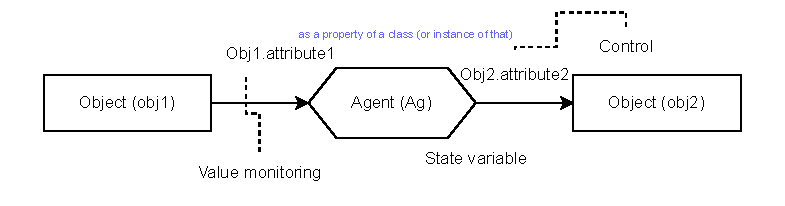
\includegraphics[width=0.8\textwidth]{assets/agent_capabilities.drawio.pdf}
    \caption{نمودار توانایی یک عامل}
\end{figure}

\subsection{وظایف عامل یا \lr{Agent responsibilities}}

در این حالت می‌توانیم مشخص کنیم که عامل دقیقاً چه کاری را باید نسبت به رسیدن و
محقق شدن هدف انجام دهد.

\begin{figure}[H]
    \centering
    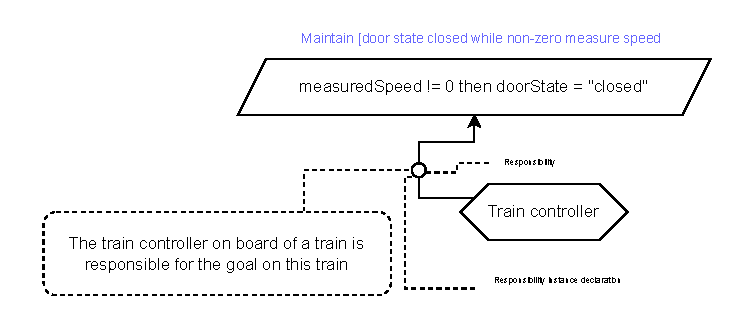
\includegraphics[width=0.8\textwidth]{assets/agent_responsibilities.drawio.pdf}
    \caption{نمودار مسئولیت یک عامل}
\end{figure}

\subsection{وابستگی‌های عامل یا \lr{Agent dependencies}}

زمانی که عوامل برای محقق کردن اهداف تعریف شده خود به یکدیگر وابسته باشند، به
گونه‌ای که اگر عوامل بالایی قادر به انجام مسئولیت و وظیفه خود نباشند، وابستگی
عامل اول به عامل دوم نیز وجود دارد و این باعث می‌شود که عامل اول به خاطر ضعف
انجام مسئولیت عامل دوم به هدف مورد نظر خود نرسد. معمولاً از این بخش به عنوان
زنجیره تحمیل نیز یاد می‌شود.

\begin{figure}[H]
    \centering
    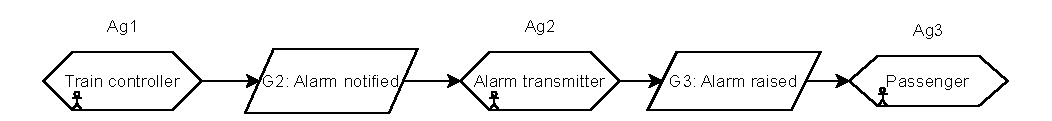
\includegraphics[width=0.8\textwidth]{assets/agent_dependencies.drawio.pdf}
    \caption{نمودار زنجیره آسیب}
\end{figure}

کنترلر قطار به عامل \lr{Alarm transmitter} برای اعلان آلارم وابسته است. همچنین
عامل \lr{Alarm transmitter} به عامل (کاربر یا مسافر) وابسته است که دکمه آلارم را
بفشارد (یا به اصطلاح باعث فراخوانی تابع \lr{alramRaised}) شود.

نکته مهم در این دیاگرام آن است که حتماً در ابتدا به یک هدف مشخص متصل است و مهندس
نیازمندی آن را از «انتها به ابتدا» می‌خواند.

مدل‌های عامل محور را می‌توانیم با سه نمودار نمایش دهیم:

\begin{enumerate}
    \item \lr{Agent diagram}: کامل‌ترین نمونه می‌باشد که تمام عوامل اعم از
    اهداف، عوامل و کلاس‌ها را خواهیم داشت.
    \item \lr{Context diagram}: مجموعه ارتباطی میان \lr{Assumption}ها و غیره
    می‌باشد.
    \item \lr{Dependency diagram}: تعریف زنجیره آسیب می‌باشد.
\end{enumerate}

\subsection{نمودار عامل یا \lr{Agent diagram}}

تمام عوامل را با توجه به مسئولیت‌ها، قابلیت‌ها و عملیاتشان را نشان می‌دهد.

\begin{figure}[H]
    \centering
    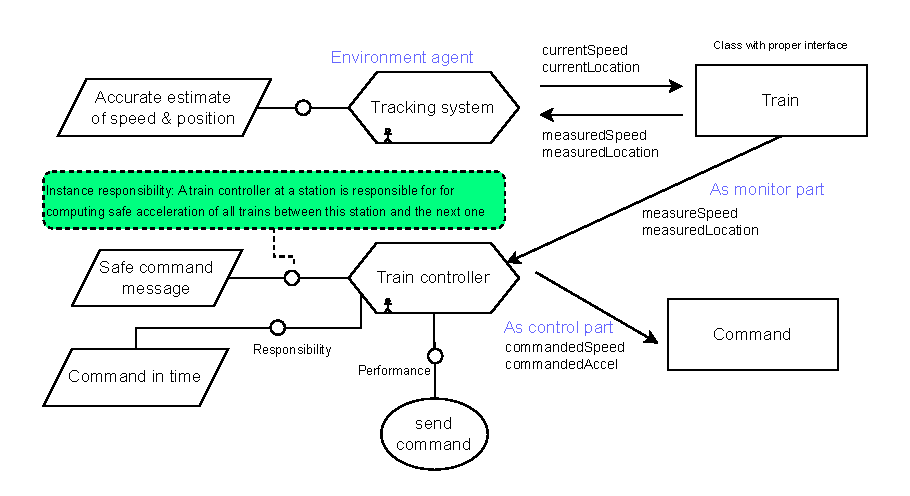
\includegraphics[width=0.8\textwidth]{assets/sample_of_agent_diagram.drawio.pdf}
    \caption{نمونه‌ای از نمودار عامل}
\end{figure}

\subsection{نمودار زمینه یا \lr{Context diagram}}

ارتباط بین \lr{Assumption} چه انسان باشد، چه سخت‌افزار و چه نرم‌افزار‌های موجود
(\lr{Library and packages}) را نشان می‌دهد.

\begin{figure}[H]
    \centering
    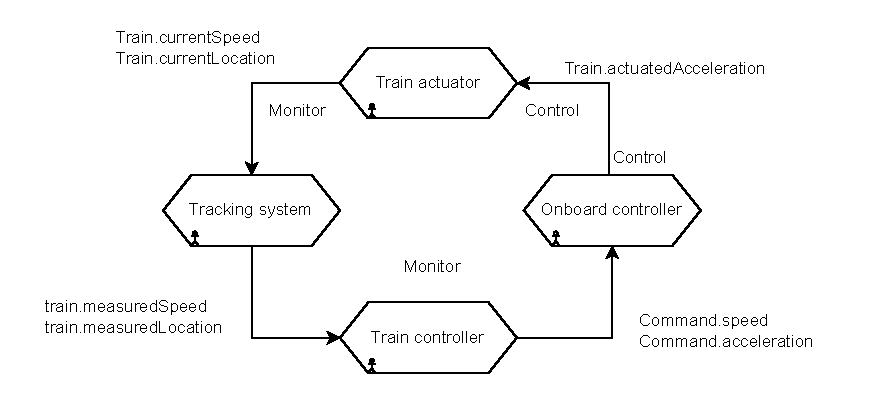
\includegraphics[width=0.8\textwidth]{assets/sample_of_context_diagram.drawio.pdf}
    \caption{نمونه‌ای از نمودار زمینه}
\end{figure}

\subsection{نمودار وابستگی یا \lr{Dependency agent}}

عواملی که نسبت به انجام کار خود به عوامل قبلی خود وابسته هستند را به وضوح نمایش
می‌دهد.
